% $Id:
% !Mode:: "TeX:DE"    % Setting document mode and submode for WinEdt
% ..............................................................................
%         H o m o m o r p h e   C h i f f r e n
% ~~~~~~~~~~~~~~~~~~~~~~~~~~~~~~~~~~~~~~~~~~~~~~~~~~~~~~~~~~~~~~~~~~~~~~~~~~~~~~

\begin{refsegment}

\newpage
% #### old naming: \hypertarget{homciph}{}
\hypertarget{Chapter_HomomorphicCiphers}{}
\chapter{Homomorphe Chiffren}
\label{Chapter_HomomorphicCiphers}
\index{homomorphe Chiffren}\index{Verschlüsselung!homomorph}
(\hyperlink{author_Martin-Franz}{Martin Franz}, Januar 2013)

% -----------------------------------------------------------------------------
\section{Einführung}

Homomorphe Chiffren sind Public-Key-Verfahren mit besonderen Eigenschaften. Sie erlauben es, bestimmte Berechnungen auf verschlüsselten Daten durchzuführen, ohne die Daten selbst zu kennen oder diese entschlüsseln zu müssen. Dies findet in der Praxis relevante Anwendungen, z.B. im Bereich Cloud-Computing. Ein sehr bekanntes homomorphes Kryptosystem ist das von Paillier. Aber auch ältere Kryptosysteme wie das von ElGamal oder RSA besitzen homomorphe Eigenschaften.


% -----------------------------------------------------------------------------
\section{Ursprung und Begriff \glqq homomorph\grqq}

Zunächst klären wir den Ursprung des Begriffs\glqq homomorph\grqq. Dieser stammt aus der Mathematik: Hier bezeichnet ein Homomorphismus eine Struktur-erhaltende Abbildung zwischen zwei algebraischen Strukturen. Umgangssprachlich gesagt bildet ein Homomorphismus $f: X \to Y$ dabei die Struktur von $X$ auf die von $Y$ ab. An einem Beispiel lässt sich dies sehr gut verdeutlichen. Seien $(X,+)$ und $(Y,*)$ zwei Gruppen mit den Operationen $+$ bzw. $*$. Ein Homomorphismus $f: X \to Y$ bildet nun jedes $x \in X$ so auf ein $y \in Y$ ab, dass gilt:
$$f(x_1 + x_2) = f(x_1) * f(x_2)$$
für beliebige $x_1, x_2$ aus $X$. Es spielt also für die beiden Werte $x_1, x_2$ keine Rolle, ob man sie zunächst addiert (Gruppenoperation von $X$) und dann $f$ anwendet (linke Seite der Gleichung); oder ob man zuerst  $f$ auf die beiden Werte $x_1, x_2$ anwendet, und dann die Gruppenoperation von $Y$, die Multiplikation, anwendet. Die Operationen $+$ bzw. $*$ wurden hier nur beispielhaft verwendet, sie hängen immer von der jeweiligen Gruppe ab. Beispielsweise gibt es auch Homomorphismen zwischen Gruppen mit derselben Gruppenoperation.
\\\\
\begin{example}{:} Nehmen wir für $X$ die Menge der ganzen Zahlen $\mathbb{Z}$, diese bilden zusammen mit der Addition eine Gruppe $G_1 = (\mathbb{Z}, +)$. Genauso bilden die reellen Zahlen ohne Null zusammen mit der Multiplikation eine Gruppe $G_2 = (\mathbb{R}\backslash\{0\}, *)$. Die Funktion $f:\mathbb{Z} \to \mathbb{R}\backslash\{0\},z \to e^z$ ist ein Homomorphismus, denn für alle $z_1,z_2 \in \mathbb{Z}$ gilt: $f(z_1+ z_2) = e^{(z_1+ z_2 )}=f(z_1 )* f(z_2)$. Die Funktion $f:\mathbb{Z} \to \mathbb{R}\backslash\{0\}, z \to z^2$ dagegen ist kein Gruppenhomomorphismus.
\end{example}

% -----------------------------------------------------------------------------
\section{Entschlüsselungsfunktion ist Homomorphismus}

Wir betrachten im Folgenden Public-Key-Kryptosysteme mit einer besonderen Eigenschaft: Eine Public-Key-Chiffre wird homomorph genannt, wenn ihre Entschlüsselungsfunktion ein Homomorphismus ist.

Sei nun angenommen, der obige Homomorphismus $f$ sei die Entschlüsselungsfunktion eines Kryptosystems. Das bedeutet, dass wir in der Algebra der Geheimtexte Operationen durch"-führen können und dabei wissen, welche Auswirkungen dies auf die Klartexte hat. Angewendet auf das obige Beispiel:

$Y$ ist die Menge der Geheimtexte, $X$ die Menge der Klartexte.
Für zwei Klartexte $x_1, x_2$ mit zugehörigen Geheimtexten $y_1, y_2$ gilt:

$$f(y_1  * y_2) = f(y_1) + f(y_2) = x_1  + x_2$$

Übersetzt bedeutet diese Gleichung: Multipliziere ich zwei Geheimtexte $y_1, y_2$ miteinander und entschlüssele dann deren Produkt, so erhalte ich die Summe der ursprünglich verschlüsselten Werte $x_1$ und $x_2$. Jedermann kann -- ohne Kenntnis der Klartexte und ohne Kenntnis der Entschlüsselungsfunktion -- ein Produkt zweier Geheimtexte berechnen und weiß, dass der autorisierte Entschlüsseler aus dem berechneten Produkt  die Summe der beiden ursprünglichen Klartexte erhalten wird.

% -----------------------------------------------------------------------------
\section{Beispiele für homomorphe Chiffren}

\subsection{Paillier-Kryptosystem}

Das wohl bekannteste Kryptosystem mit solchen homomorphen Eigenschaften ist das von Paillier\allowbreak\cite{Paillier1999}. Wir sehen zunächst, wie die Schlüsselerzeugung, die Verschlüsselung und die Entschlüsselung funktionieren, und zeigen dann, dass das Paillier-Kryptosystem homomorphe Eigenschaften besitzt.

\subsubsection{Schlüsselerzeugung}

Zuerst werden zwei zufällige Primzahlen $p,q$ erzeugt, so dass das Produkt $n=pq$ einen gültigen RSA-Modulus formt. Hierbei sollte $n$ eine Bitlänge von mindestens 1024 Bit haben.
Damit kann der private Schlüssel $\lambda = \textit{kgV}(p-1,q-1)$ berechnet werden. $\textit{kgV}$ bezeichnet hierbei das kleinste gemeinsame Vielfache. Der öffentliche Schlüssel besteht nur aus dem RSA-Modulus $n$.

\subsubsection{Verschlüsselung}

Sei $m$ die zu verschlüsselnde Nachricht aus dem Klartextraum $\mathbb{Z}_n$. Für jeden Verschlüsselungs"-vorgang wählen wir zunächst ein zufälliges Element $r$ aus $\mathbb{Z}_n$ und berechnen dann mit Hilfe des öffentlichen Schlüssels $n$ den Geheimtext:

$$c = E(m,r) = (n+1)^m  * r^n  \bmod n^2$$

\subsubsection{Entschlüsselung}

Sind der private Schlüssel $\lambda$ und ein Geheimtext $c \in \mathbb{Z}_{n^2}^*$ gegeben, berechnen wir zunächst
$$S = c^\lambda \bmod n^2 \mbox{ und } T = \phi(n)^{(-1)} \bmod n^2,$$
wobei $\phi$ die Eulersche Funktion ist.
Und dann $m = D(c) = (S-1)/n * T \bmod n$.

\subsubsection{Homomorphe Eigenschaft}

Um die homomorphe Eigenschaft nachzuweisen, betrachten wir die Verschlüsselungsfunktion $E$ und die Entschlüsselungs"-funktion $D$ des Paillier-Kryptosystems. Zur Vereinfachung setzen wir im Folgenden $g:= n+1$.  Aus zwei Klartexten $m_1,m_2$ ergeben sich die dazugehörigen Geheimtexte $c_1, c_2$ als
$$c_1 = g^{m_1} *  {r_1}^n \bmod n^2 \mbox{ bzw. } c_2 = g^{m_2} * {r_2}^n \bmod n^2$$
Wir sehen, dass für das Produkt $c_3 = c_1 * c_2$ gilt
$$c_3 = (g^{m_1} * {r_1}^n \bmod n^2) * (g^{m_2} * {r_2}^n \bmod n^2) = g^{m_1+m_2} * (r_1*r_2 )^n \bmod n^2 = E(m_1 + m_2, r_1*r_2)$$
Das Produkt zweier Geheimtexte ist also wieder ein Geheimtext, und zwar eine Verschlüsselung der Summe der ursprünglichen Nachrichten. Nun ist es leicht zu sehen, dass die Ent"-schlüsselungs"-funktion ein Homomorphismus ist:
Gegeben zwei Klartexte $m_1, m_2$ dann gilt
$$D( E(m_1,r_1) * E(m_2,r_2)) = D( E(m_1+m_2, r_1 r_2)) = m_1  + m_2 = D(E(m_1,r_1)) + D(E(m_2,r_2))$$

\subsection{Weitere Kryptosysteme}

Auch ältere Public-Key-Kryptosysteme können homomorphe Eigenschaften haben. Das ElGamal"--Krypto"-system und das Standard RSA-Kryptosystem sind bekannte Beispiele dafür. Wir zeigen diese homomorphen Eigenschaften anhand einfacher Beispiele auf.

\subsubsection{RSA}

Sei $(e,n)$ der öffentliche RSA-Schlüssel ($e$ der Verschlüsselungskoeffizient, $n$ der RSA-Modulus). Für zwei Nachrichten $m_1, m_2$ erhält man die Verschlüsselungen $c_1 = {m_1}^e \bmod n$ und $c_2 = {m_2}^e \bmod n$. Nun gilt für das Produkt dieser beiden Verschlüsselungen: $c_1*c_2={m_1}^e * {m_2}^e \bmod n=(m_1*m_2)^e \bmod n$. Man erhält also eine Verschlüsselung des Produkts der ursprünglichen Nachrichten. Wie man leicht nachprüfen kann gilt diese Eigenschaft für beliebige Nachrichten $m_1, m_2$, somit ist die Entschlüsselungsfunktion ein Homomorphismus. RSA ist dabei ein Beispiel für einen Homomorphismus, bei dem in beiden Gruppen die gleiche Gruppenoperation verwendet wird.

\subsubsection{ElGamal}

Ähnlich wie bei RSA verhält es sich auch im ElGamal-Kryptosystem. Sei $(p,g,K)$ der öffentliche Schlüssel, der private Schlüssel sei $k$ (es gilt also $g^k \bmod p = K$). Für Nachrichten $m_1, m_2$ erhält man nun Verschlüsselungen $(R, c_1) = (K^r \bmod p, m_1*g^r \bmod p)$ und $(S,c_2) = (K^s \bmod p, m_2 * g^s \bmod p)$. Auch hier ist das Produkt $(R*S, c_1*c_2)$ eine Verschlüsselung von $m_1*m_2$ und man kann leicht überprüfen, dass die Entschlüsselungsfunktion ein Homomorphismus ist.

% -----------------------------------------------------------------------------
\section{Anwendungen}
Die homomorphe Eigenschaft lässt sich dazu verwenden, um verschlüsselte Werte zu addieren oder verschlüsselte Werte mit unverschlüsselten Werten zu multiplizieren (dies entspricht einer wiederholten Anwendung der Addition). Damit werden homomorphe Chiffren zu einer wichtigen Funktion in vielen kryptographischen Anwendungen.

\begin{enumerate}
\item Eine dieser Anwendungen ist das sogenannte \glqq Electronic Voting\grqq. Hierbei wird es mehreren Wahlberechtigten ermöglicht, ihre Stimme verschlüsselt abzugeben. Dies ist wichtig in Situationen, in denen die Wahlberechtigten nicht direkt zusammen kommen können. Zum Beispiel könnte es sein, dass die Wahlberechtigten nur per Email über das Internet kommunizieren können. Wenn die Abstimmung geheim bleiben soll, und es niemanden gibt, dem alle Wahlberechtigten uneingeschränkt vertrauen, bieten homomorphe Chiffren eine gute Lösung für dieses Problem. Im Wesentlichen funktioniert Electronic Voting mittels homomorpher Chiffren so:

\begin{itemize}
\item Alle Wahlberechtigen (links in der Abbildung \ref{CT2-PaillierVoting}) verschlüsseln ihre Stimme. Sie verschlüs"-seln den Wert 1, wenn sie für die Entscheidung sind, und den Wert 0, wenn sie dagegen sind.
\item Über die homomorphe Eigenschaft wird die Summe der abgegebenen Stimmen berechnet. Da dies auf den verschlüsselten Werten passiert, bleiben die Stimmen der einzelnen Wahlberechtigten geheim.
\item Am Ende werden die Stimmen ausgezählt, indem nur die Summe der Stimmen entschlüsselt wird.
\end{itemize}

\begin{figure}[ht]
\begin{center}
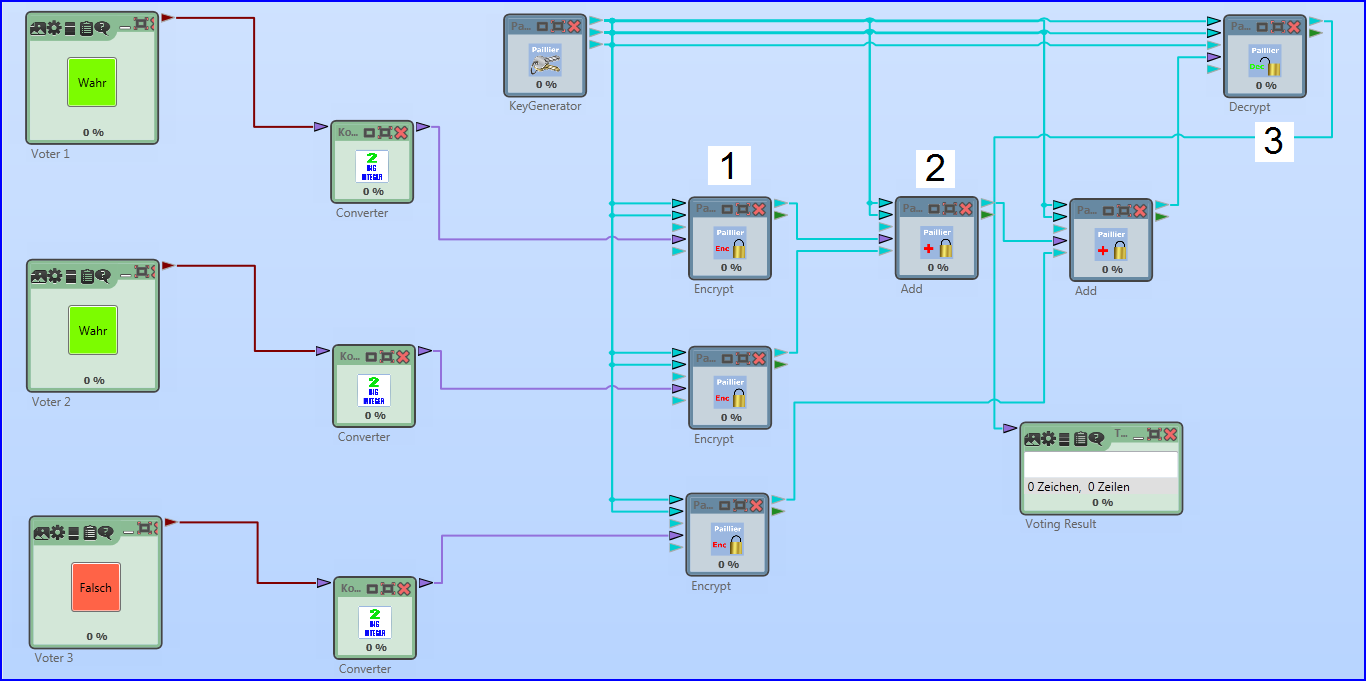
\includegraphics[scale=0.4]{figures/CT2-PaillierVoting.png}
\caption{Voting-Beispiel für Paillier}
\label{CT2-PaillierVoting}
\end{center}
\end{figure}

\item Ein weiteres Anwendungsgebiet für homomorphe Chiffren ist \glqq Secure Multiparty Computation\grqq. Hierbei berechnen mehrere Parteien gemeinsam eine vorgegebene Funktion. Jede der Parteien steuert einen Input für die zu berechnende Funktion bei. Das Ziel der Berechnung ist es, alle Inputs und auch die Zwischenergebnisse geheim zu halten, während nur das Ergebnis der Funktion bekannt wird. Die Verwendung homomorpher Chiffren hilft dabei, diese Berechnungen auf verschlüsselten Daten durchzuführen. Da sich allerdings unter der homomorphen Chiffre von Paillier nur Additionen (und z.B. keine Multiplikationen durchführen lassen), müssen noch weitere geeignete Methoden verwendet werden. Einen guten Einstieg in dieses Thema bietet Wikipedia \cite{Wiki_SMC}.

\item Weiterhin wird erwartet, dass homomorphe Chiffren im Bereich Cloud Computing enorme Vorteile bringen können. Mittels sogenannter voll-homomorpher Kryptosysteme \cite{Wiki_HomEnc} wird es möglich sein, komplette Anwendungen auf verschlüsselten Daten durchzuführen. Hierzu ist es notwendig, dass unter der homomorphen Verschlüsselung die beiden Operationen Addition und Multiplikation durchgeführt werden können (im Gegensatz zum Paillier-Kryptosystem, welches nur die Addition unterstützt). Ein solches Kryptosystem wurde erstmals 2009 von Craig Gentry vorgestellt \cite{Gentry2009}.
\end{enumerate}

% -----------------------------------------------------------------------------
\section{Homomorphe Chiffren in CrypTool}

\subsection{CrypTool~2}
In CrypTool~2\index{CT2} findet man bereits eine Implementierung des Paillier-Kryptosystems (siehe Bild \ref{CT2-Paillier}). Unter den fertigen Vorlagen finden sich Methoden zur Erzeugung der kryptographischen Schlüssel (Paillier Key Generator), ein Beispiel für eine Ver- und Entschlüsselung mittels Paillier (Paillier Text), sowie Beispiele, die die homomorphen Eigenschaften von Paillier aufzeigen (Paillier Addition, Paillier Blinding und Paillier Voting).

\begin{figure}[ht]
\begin{center}
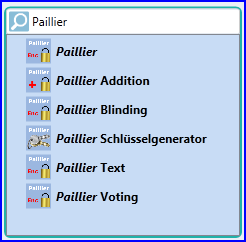
\includegraphics[scale=0.8]{figures/CT2-Paillier.png}
\caption{Paillier-Kryptosystem in CrypTool~2 (CT2)}
\label{CT2-Paillier}
\end{center}
\end{figure}

\newpage

\subsection{JCrypTool}

Im JCrypTool\index{JCT} gibt es eine Implementierung (siehe Bild \ref{JCT-HomEnc}), die die homomorphen Eigenschaften verschiedener Kryptosysteme visualisiert. Für RSA und Paillier wird gezeigt, dass jeweils Multiplikationen (für RSA) und Additionen (für Paillier) auf verschlüsselten Werten möglich sind. Für das voll-homomorphe Kryptosystem von Gentry können sowohl Multiplikationen als auch Additionen auf verschlüsselten Werten durchgeführt werden.

\begin{figure}[ht]
\begin{center}
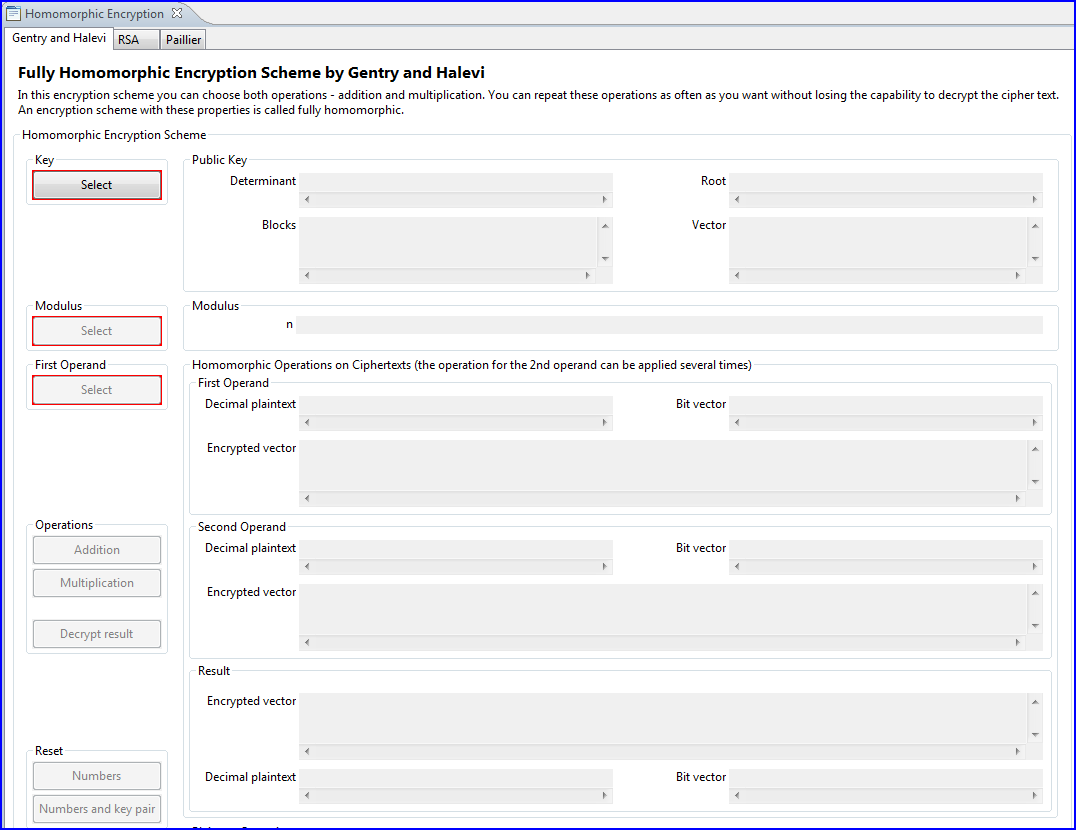
\includegraphics[scale=0.4]{figures/JCT-HomEnc.PNG}
\caption{Kryptosysteme mit homomorphen Eigenschaften in JCrypTool (JCT)}
\label{JCT-HomEnc}
\end{center}
\end{figure}



%------------------------------------------------------------------------------
\printbibliography[%
	heading=subbibintoc,
	title={Literatur zu Kapitel \thechapter},
	segment=\therefsegment,
]


\noindent Alle Links im Artikel wurden am 15.07.2016 überprüft.


\end{refsegment}

% Local Variables:
% TeX-master: "../script-de.tex"
% End:
